
% Zitat: Auf den Schultern von Riesen.

This chapter will give an introduction into the basics needed to
follow this thesis. We will be introduced into functional programming
in Haskell to ease the understanding of the presented code.
Then we will cover Nested Data Parallelism (NDP) where
key insights - and concepts to make use of them - will be presented.
Afterwards a short introduction into parallel complexity measures is given.
We will learn about work and depth complexities, how they relate
to the runtime duraiton and how they can be calculated.
Finally, the problem of \algo itself is presented - along with
a description on how it works and examples for its uses in image processing.

\section{Haskell}
  introduction into syntax, immutability, and higher-order functions, lambdas, currying
  polymorphic types (PA a, Dist a, Vector a), type synonyms,
  type safety!!
  evaluation, record syntax, naming conventions functions f,g,h, vars x,y,z,a,b,c, arrays of x -> xs -> xss
  identity function, flip
  
  Quick guide of Haskell!


\section{Nested Data Parallelism}
  In the ground breaking work \cite{Belloch1996}
  major contributions to parallel programming in
  functional programming languages were made.
  The paper presented some of Belloch's earlier work (\cite{NepaBelloch1993}) on NESL
  - a programming language specifically designed for expressing parallelism
  in functional programming languages. Its ideas and insights were
  adapted to various languguages - one of them being Haskell.
  Multitude years of research was nesessary to generalize the
  advantages of the special purpose language NESL to a widely used
  general purpose language like Haskell.
  \footnote{For example \cite{Harness2008}, \cite{DPHStatus2007},
  \cite{EffiVect2012Lipp}, \cite{HighOrdFlat2006} and \cite{DistTypes1999}.}
  This project is called Nested Data Parallel Haskell and this section will give
  an overview of its key concepts.  
  
  \paragraph{}
    In Flat Data Parallelism, we are provided with parallel mapping primitives
    to express parallelism. For example, we might have a built-in
    function \c{map} such that \c{map f xs} applies \c{f}
    on each of the elements in the array \c{xs} in parallel.
    
    This function has a farily intuitive parallel implementation -
    simply distribute the input array evenly across the \underline{p}rocessing \underline{u}nits (PUs),
    compute each local chunk of the array with its PU and finally
    join all elements together.
    The inner function \c{f} is applied by each processing unit (PU) individually.
    It is therefore executed sequentially.
    
    This is no problem, if we have statements like \c{mapm incr}
    \footnote{where \c{incr} increments an integer.}
    . However, what shall we do if we have an expression like \c{map (mapm incr)}?
    Or even \c{map (map (mapm incr))}?
    We can only execute the outermost level in parallel because we have already
    distributed the workload among the PUs.
    That means, that the inner function \c{f} can only be executed squentially.
    
    
    This is where NDP can shine. In NDP, in contrast, \c{f} itself can
    also be a parallel operation - and all levels of nesting can
    be executed in parallel! Hence the name - \textbf{Nested} Data Parallelism.
    It does that by transforming the program we wrote into a functionally
    equivalent flat data parallel program. This (non-trivial) transformation
    is called 'flattening' or 'vectoriation' and subsequent optimisations.
    All in all the entire program transformation can be broken down in three steps.
    Each step introduces it own new data types.
    \begin{enumerate}
      \item \emph{Vectorization} -
        Uses flat type-dependent array \pav representations instead of the
        vanilla nested parallel arrays \pan which are used by the programer.
        The flatening is also applied to nested parallelism.
      \item \emph{Communicaiton Fusioning} -
        By inlining the definitions of the parallel functions and
        using semantics-preserving rewrite rules one can
        reduce unsessesary synchronisation points and
        create tight pipelines. It uses \pad to denote
        distributed chunks of a global array \pav.
      \item \emph{Stream Fusioning} -
        Sequential functions local to each PU can further
        be optimised similarly to the previous step
        to reduce the number of intermediate arrays and
        to create tight loops.
        It uses \type{Vector a} and \c{Stream a} to
        implement the local array chunks and to fuse loops, respectively.
    \end{enumerate}
    
  After a overview of the predefined functions - these steps
  are going to be explained in more detail.
  
  \paragraph{}
    For parallel arrays, we have a few predefined operations availible.
    They correspond to functions used in conventional functional programming.
    Their names and their types are given in \ref{table:parfuncs}.
    
    \begin{table}[h]
      \caption{Table of functions}
      \label{table:parfuns}
      \begin{tabular}{lll}
          \toprule
          function & type & description \\
          \midrule
          (!:),indexP & \c{[:a:] -> Int -> a} & indexing \\
          lengthP & \c{[:a:] -> Int} & return the length of the array \\
          headP & \c{[:a:] -> a} & returns the first element\\
          lastP & \c{[:a:] -> a} & returns the second element \\
          mapP & \c{(a -> b) -> [:a:] -> [:b:]} & apply a function on all elements \\
          sortP & \c{[:Int:] -> [:Int:]} & sorts an array \\
          concatP & \c{[:[:a:]:] -> [:a:]} & remove a level of nesting \\
          unconcatP & \c{[:[:a::]] -> [:b:] -> [:[:b:]:]} & expose a structure to a flat array \\
          replP & \c{Int -> a -> [:a:]} & replicate an element \\
      \end{tabular}
    \end{table}

    
  \subsection{Vectorization}
    Vectorization roughly involves two major steps -
    \emph{Type dependent representation} and \emph{Lifting}.
    Both will be explained in detail now.
  
    \subsubsection{Type dependent representation}
      Type dependent representation 
      allows the programer to work with arrays containing complex
      data structures without sacrifying efficiency.
      
      Consider for example \type{[:Int:]} and \type{[:[:Int:]:]}.
      The former can be easily implemented using a contiguos region
      of memory and inserting the bytes. The latter however cannot
      be implemented equally. What if the sub-arrays are of unequal length?
      To allocate a block of memory, we need to know the size
      of all arrays beforehand.
      Implementing nested array naively would use an array of pointers to
      to arrays of integers. Pointers however are bad, since they
      decrease cache locality and therefore decrease overall performance.
      How can we implement a nested array without using many pointers?
      
      The solution is separation of data and structure.
      The folowing example describes how a nested array
      like \c{[[1,2,3],[4,5],[],[6]] :: [:[:Int:]:]} would be implemented:
      \footnote{\c{[#1,2,3#]} is the notation used for a contiguos-memory array.}
      \begin{lstlisting}
array :: PA (PA Int)
array = AArr {
  data = [# 1,2,3,4,5,6 #],
  indices = [# 0,3,5,5 #]
  lengths = [# 3,2,0,1 #]
}
      \end{lstlisting}
      All data is packed together into a data field - regardless nesting -
      and all structucal information is divied into two byte-arrays.
      The indices describe the index in the data field of the first element
      of each subarray. The lengths describe the lengths of
      each subarray. Each subarray corresponds to a pair of index and length.
      For example, the second subarray (\c{[4,5]}) corresponds to
      the second index (3) and second length (2). Extracting
      2 elements starting at index 3 in the \c{data} array will return
      exactly these two elements.
      Another thing to note is, that this flat representation
      also uses the new type \type{PA (PA Int)}
      instead of the old \type{[:[:Int:]:]}.
      
      There are implementation for all other types - such as arrays of ints.
      For example \c{[:1,2,3:] :: [:Int:]} can be simply
      represented as:
      \begin{lstlisting}
array :: PA Int
array = AInt [# 1,2,3 #]
      \end{lstlisting}
      
      The compiler also automatically transforms any functions \c{fooP}
      to \c{fooPS}. This is to make sure, that the new functions
      adhere to the new types of the arrays used.
    
    \nomenclature{Cache Locality}{TODO}
      
    \subsubsection{Lifting}
      During lifting where all occurrences of \c{mapPS f} are
      replaced by \c{fL} and where \c{fL}
      is the lifted version of the original function.
      \footnote{where \c{fL} has type \type{PA a -> PA b}
        if \c{f} had type \type{a -> b}
      }.
      Compared to the original scalar function \c{f :: a -> b}, the lifted
      function applies the mapping over arrays - that means \c{fL :: PA a -> PA b}
      For user defined-functions, this lifted function is defined
      by lifting the definition of \c{f} recursively.
      The key is now the definition of the lifted functions for the built-in functions.
      The most important one among them is lifted \c{mapPS} - namely \c{mapPL}.
      To \c{mapPS} of type \c{(a -> b) -> PA a -> PA b},
      \c{mapPL} is of type \c{(a -> b) -> PA (PA a) -> PA (PA b)}.
      To overcome the limitations of flat data parallelsim,
      we now have to map over all elements at once
      (instead of mapping over the outer-nesting level only).
      The following definition does that.
    \begin{lstlisting}
mapPL :: (a -> b) -> PA (PA a) -> PA (PA b)
mapPL f xss =
  unconcatPS xss
  . fL
  . concatPS
  $ xss
    \end{lstlisting}
    The definition of \c{mapPL} is curcial. It is implemented by flattening the array (line 5), applying a flat data-parallel operation (line 4)
    and finally unflattening the new array into the original structure (line 3).
    \footnote{This implementation is different from the original in one important aspect - 
    namely the handling of presupplied arguments in the function. Our
    implementation only handles functions without presupplied arguments -
    but it much simpler to understand than the original in \cite{Harness2008}.
    Introducing it wouldn't affect the overall situation in this thesis -
    so it was simplified.
    }
    Figure \ref{figure:mapP} shall visually aid the understanding by using
    and example of \c{mapP (mapP incr)}.
    
    \begin{figure}[h!]
        \begin{center}
        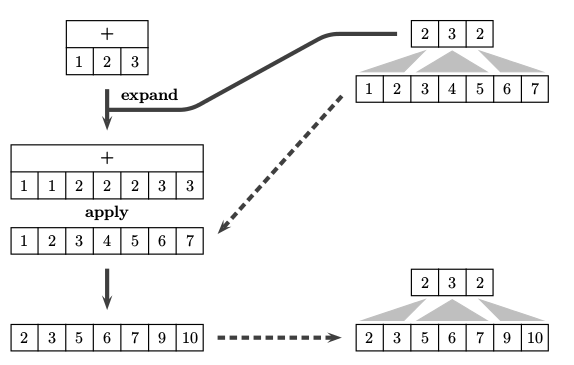
\includegraphics[width=\linewidth]{mapP.png}
        \caption{Conceptional programer view and actual implementation of \c{mapP (mapP incr)}}
        \label{figure:mapP}
        \end{center}
    \end{figure}
    
    This is the key insight in NDP! Nested Parallel operations - like \c{mapP (mapP incr)} are
    transformed into calls of \c{mapPL incrL} which avoid the nesting of
    the arrays entirely and enable us to map over the entire array in parallel.
    Using this precedure, we can transform nested data parallel programs
    to flat data parallel programs. The former is easy to wirte and flexible
    - while the latter is simple to implement.
            
    Vectorization itself is a complex transformation - and many details were ommited.
    More details can be found in \cite{Harness2008}.
    
  \subsection{Communication Fusion}
    % TODO:
    Example lifted function
    What is Dist a?
    
  \subsection{Stream Fusion}
    % TODO:
    Example streaming function
    What is Stream a?
    
  \subsection{Tables of Functions and Rewrite Rules}
    The transformation in chapter \ref{chapter:ndpv} is going to
    make use of many functions. Most of them will are going to be
    introduced when they first appear - others are more frequent
    and require a summary. They are explained in table \ref{mapPs}.
    The table also holds for other functions with same suffix - e.g.
    the \c{mapP} row similarly applies to \c{scanlP}, \c{groupP} etc.
    
    \begin{table}[h]
      \caption{Table of functions}
      \label{mapPs}
      \begin{tabular}{lll}
          \toprule
          function & first appearance/ & type/ \\
            & execution context & description \\
          \midrule
          mapP f xs & Programer-view & \type{(a -> b) -> [:a:] -> [:b:]} \\
           & not executed & \textbf{P}arallel array functions the programer uses \\
          mapPS f xs & Vectorization & \type{(a -> b) -> PA a -> PA b} \\
           & not executed & \textbf{P}arallel \textbf{S}calar functions the program is vectorized into \\
          indexPL is xs & Vectorization & \type{PA Int -> PA (PA a) -> PA a} \\
           & not executed & \textbf{P}arallel \textbf{L}ifted indexing on flat arrays. It's scalar\\
           & & function is \type{indexP :: Int -> [:a:] -> a} \\
          mapD f x & Communication Fusion & \type{(a -> b) -> Dist a -> Dist b} \\
           & mapD: all PUs & Each PU applies \c{f} on it's chunk of the \\
           & f: local per PU & \textbf{d}istributed value. True parallelsim here! \\
          mapS f xs & Communication Fusion & \type{(a -> b) -> Vector a -> Vector b}\\
           & local PU & Applies a mapping \textbf{s}equentially. \\
           & & \c{Vector} is the Haskell implementation of \\
           & & conventional local in-memory arrays. \\
          splitD & Communication Fusion & \type{PA -> Dist (PA a)}\\
           & all PUs & splits an array into chunks and \\
           & & distributes them to each of the PUs \\
          joinD & Communication Fusion & \type{Dist (PA a) -> PA a}\\
           & all PUs & joins local chunks into a global array \\
          mapSt f xs & Stream Fusion & \type{(a -> b) -> Stream a -> Stream b}\\
           & not executed & Applies a function on a \textbf{st}ream of values \\
      \end{tabular}
    \end{table}

    \nomenclature{\c{Vector}}{is the Haskell implementation of conventional local in-memory arrays.
            They are used as the distributed chunks of \pad.}
    
    Most of the functions are simply inlined during optimisation.
    They don't exist anymore at runtime and
    therefore are marked 'not-executed'. Besides these functions, we will also need handful rewrite rules.
    The most important of them are described in table \ref{rules}.
    
    \begin{table}[h]
      \caption{Table of Rewrite Rules}
      \label{rules}
      \begin{tabular}{lll}
          \toprule
          rule & rewrite & description \\
          \midrule
          splitD/joinD & splitD . joinD = id & Joining and spliting an distributed array  \\
          & & doesn't change the contents. Therefore \\
          & & it is equivalent to doing nothing. \\
          
          mapD/replD & mapD f . replD n & Replicating a value and mapping \\
          & = replD n . f & all values is equivalent to \\
          & & directly applying the function and \\
          & & subsequently replicating it. \\
          
          splitD/replPS & splitD . replPS n & Replicating and spliting a value \\
          & = replD n & is equivalent to creating the local chunks\\
          & & directly. ReplD implements this and knows \\
          & & which chunk its PU is responsible for. \\
          
          ZipReplSplit & zipWithD f (replD a) & Zipping with a replicated value\\
          & . splitD  & already in scope - is equivalent to - applying \\
          & = mapD (f a) & the mapping with the value \\
          & & curried into the function.\\
          
          mapD/zipWithD & mapD f . zipWithD g xs = & A map operation after a zip operation \\
          & zipWithD (\lam x y -> f (g x y)) xs & is equivalent to a single zip operation \\
          & & which applies both \c{f} and \c{g}. \\
          
          unstream/stream & unstream . stream = id & Converting back and fourth is \\
          &  & equivalent to doing nothing. \\
       \end{tabular}
    \end{table}
  
  % TODO: "Explicit calls to AArr and ATup2 and such mean global communication"
  % TODO: "Types of PAs are global. Types of Dist are local."
  
  
  \subsection{A word on accuracy}
    The project of NDP in Haskell is - even after 15 years -
    still in \textit{work in progress}. Due to frequent changes,
    the papers often use conflicting notation and refer to
    different statuses of progress. Inconsistent literature and a project still in work makes it difficult
    to apply it in a thesis. It is not simple to use the original ideas from
    NESL directly on Haskell as there are great differences (not mentioning
    the fact it already took 15 years to adapt).
    
    Therefore, in this thesis, I have improvised on various conflicting or
    missing details. I assumed implementations which could really have been
    used in NDP.\footnote{E.g. \c{groupP} as introducted in chapter 5 doesn't
    even exist right now. Its implementation as described is however perfectly possible.}
    The reader is hereby noted that the details
    mentioned here are implementable - but not nesessarily an accurate
    representation of the current state of progress.
    
    
  \paragraph{}
    We have now finally been introduced to the details of NDP and
    are now ready to proceed. The new sections will explain
    parallel complexitiy measures and the problem \algo itselfs.
  
  % TODO: needs citations.

    
  
  Show that GHC supports Inlining and Fusion through Rewrite Rules.
\section{Parallel Computing and Complexity Measures}
  Explain Work and Depth Complexity measures
  Give and their definitions!
   sumP implementierung als Beispiel für Laufzeiteinschätung mit Work/Depth und Anzahl von Prozessoren #1!
   
   % Nennen, dass naives stream fusioning die parallelität verliert)
  
  % cite: Parallel Programming Algorithms, NESL, Guy Belloch.
   
\section{\algo}

  Introduction into Histogram Balancing.
  
  Prefix sum is a very common operation in computer science. It is a special
    case of scanning through a ordered container from left ro right applying a binary
    associative function \c{f}.
    It is defined as:
      $$ scanl(f,z,[a_1,a_2,...,a_n])
         := [f(z,a_1),f(f(z,a_1),a_2),...,f(f(...f(f(z,a_1),a_2)...,a_{n-1}),a_n)]
      $$
    An example shall be $scanl(+,0,[1,2,2,3,-2]) = [1,3,5,8,6]$. In some definitions
    the first element is $z$. This is however not the definition we need here.
    
  
  Uses thereof and overview of an algorithm.
  Wird z.B im Zusammenhang mit \mu-Momenten zur Erkennung
    affin-transformierter Bildpaare verwendet.
